\documentclass[a4paper, 11pt]{article}
\usepackage[utf8]{inputenc} % Change according your file encoding
\usepackage{graphicx}
\usepackage{url}
\usepackage{booktabs}
\usepackage{float}
\usepackage{fancyvrb}
\graphicspath{{../}}


%opening
\title{Seminar Report: seminar Opty}
\author{Rodrigo Arias Mallo}
\date{2017U2}

\begin{document}

\maketitle

\section{Introduction}

This seminar consists of a set of experiments of a Erlang server implementing a 
optimistic concurrency control, with backward validation, to access a database. 

\section{Work done}

Some experiments have been designed to measure how different parameters affect 
the performance of the server.

Each experiment that shares the same source code is designed by a number. Each 
subexperiment where only the parameters are changed, belongs to the same 
experiment number, and is identified by a letter. This structure allows batch 
processing of all the experiments, and a change in the source code automatically 
produces an update on the subexperiments.

This hierarchy is controlled by Makefiles, which are programed to run all the 
experiments, produce the figures, and compile this document with the results in 
figures.

This design provides reproducible results. Some deviation may occur, as the seed 
was not fixed, and the concurrent process behavior is not predictable.

\newpage
\section{Experiments}

In all the experiments the average of the success rate is plotted by a line, and 
also the standard deviation in the success rate of each client. For each 
measurement, there are some comments about the explanation of the system based 
on the observed behavior.

\subsection{Experiment 1}

Some set of experiments are performed to measure the performance of the 
transaction server. Each experiment is designed by a name like 
\texttt{exp1$\alpha$} where $\alpha$ is a letter.

\begin{table}[H]
\centering
\begin{tabular}{c c c c c c}
\toprule
Exp.						&	Clients	&	Entries	&	Reads & Writes	& Time (s)	\\
\midrule
\texttt{exp1a}	&	$C$			&	10			& 10		&	10			&	3					\\
\texttt{exp1b}	&	10			&	$E$			& 10		&	10			&	3					\\
\texttt{exp1c}	&	10			&	10			& $R$		&	10			&	3					\\
\texttt{exp1d}	&	10			&	10			& 10		&	$W$			&	3					\\
\texttt{exp1e}	&	10			&	10			& 10		&	10			&	$T$				\\
\texttt{exp1f}	&	10			&	10			& $i$		&	$20-i$	&	3					\\
\bottomrule
\end{tabular}
\end{table}

With $C,E,R,W \in [1,20]$, $T \in [1,10]$ and $i \in [0,20]$.

\paragraph{\texttt{exp1a}: Clients vs Success rate.}

As more clients try to access the database more transactions conflicts appear, 
so the average success rate decreases as they grow. Also, the success rate for 
each client is similar between clients.

\begin{figure}[H]
\centering
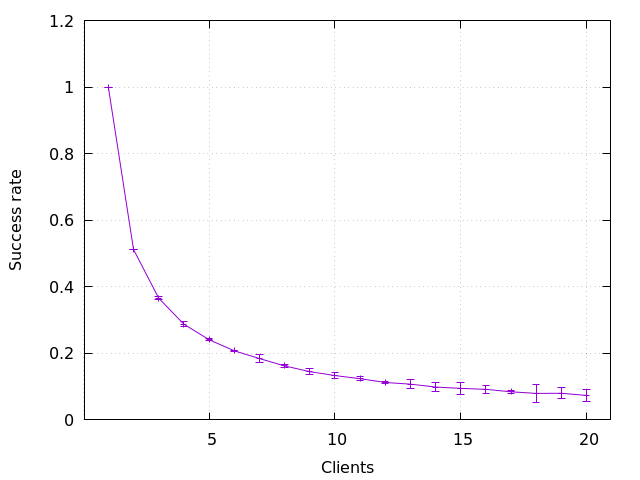
\includegraphics[width=.8\linewidth]{exp1/a/fig.png}
\end{figure}

\paragraph{\texttt{exp1b}: Entries vs Success rate}

The average success rate decreases as the entries grow, until they reach the 
value 10. Then, the success rate starts to grow slowly. We observe a increasing 
deviation in the success rate with 3 and 4 entries. The other runs show small 
deviations.
\nopagebreak
\begin{figure}[H]
\centering
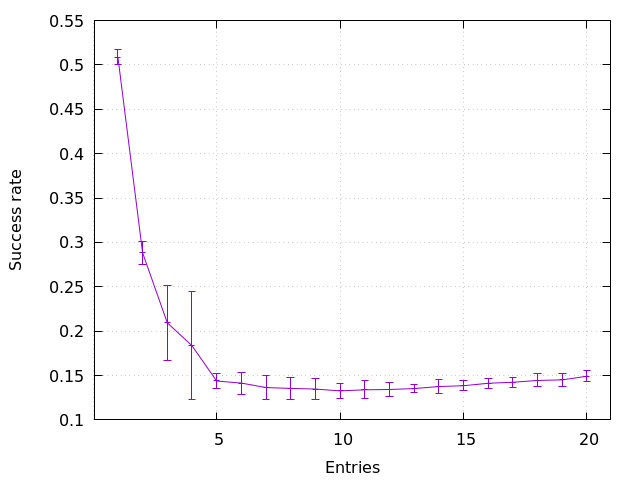
\includegraphics[width=.8\linewidth]{exp1/b/fig.png}
\end{figure}

\paragraph{\texttt{exp1c}: Reads vs Success rate}

As the number of reads performed by the clients increases, more transactions are 
in conflict, so the success rate is reduced. The deviation increases as the 
number of reads increases.
\nopagebreak
\begin{figure}[H]
\centering
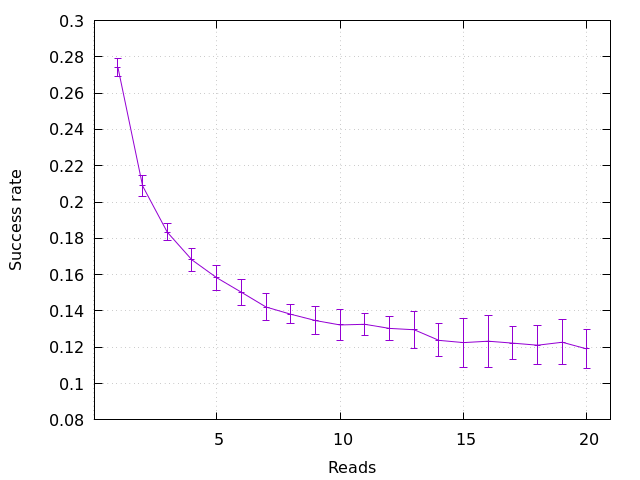
\includegraphics[width=.8\linewidth]{exp1/c/fig.png}
\end{figure}

\paragraph{\texttt{exp1d}: Writes vs Success rate}

As the number of writes performed by the clients increases, more transactions 
are in conflict, so the success rate is reduced. The deviation increases with 
the number of writes.
\nopagebreak
\begin{figure}[H]
\centering
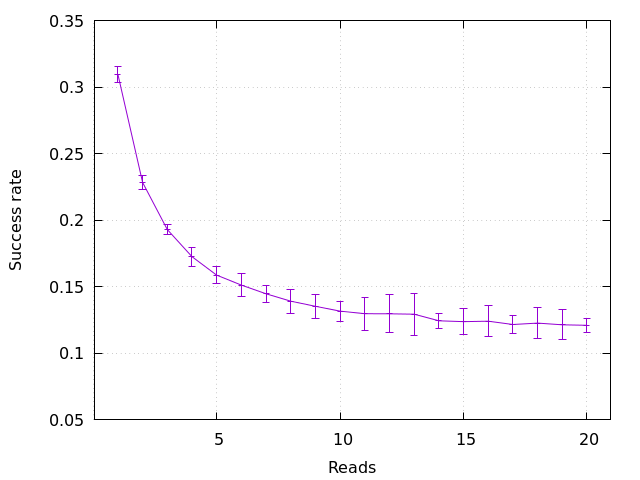
\includegraphics[width=.8\linewidth]{exp1/d/fig.png}
\end{figure}

\paragraph{\texttt{exp1e}: Time vs Success rate}

As the time allowed to the simulation grows, there seems that the success rate 
is not affected. The deviation seems to decrease as the time grows.
\nopagebreak
\begin{figure}[H]
\centering
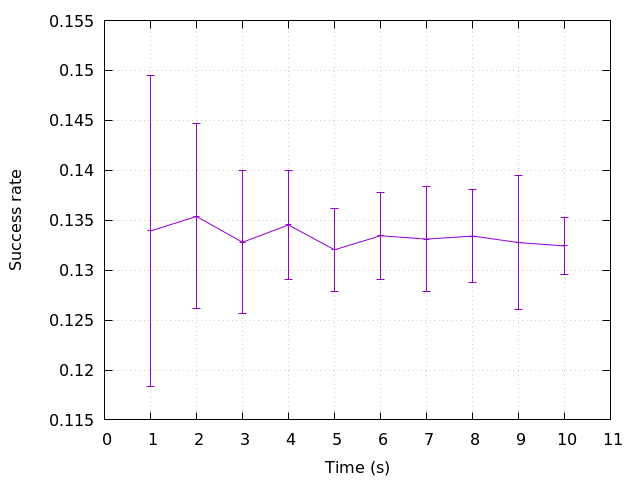
\includegraphics[width=.8\linewidth]{exp1/e/fig.png}
\end{figure}

\newpage
\paragraph{\texttt{exp1f}: Ratio R/W vs Success rate}

Let $R$ be the number of reads, then the number of writes is defined as $W = 20 
- R$.  When the number of reads or writes is 0, we have no conflicts.  But as 
the ratio is close to $1/2$ the performance is worse.  The deviation is small.
\nopagebreak
\begin{figure}[H]
\centering
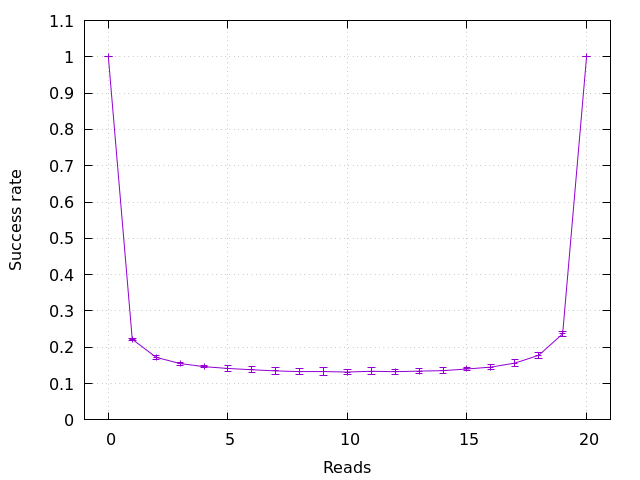
\includegraphics[width=.8\linewidth]{exp1/f/fig.png}
\end{figure}

\subsection{Experiment 2}

The experiment \texttt{exp2a} modifies the behavior of the client in order to 
access only a random subset of the entries of the database. Each client 
maintains a subset of size $A$, which is randomly selected from all the entries.
The size of the subset $A$ is tested with values in $[1, 20]$ for a database of 
20 elements.

\newpage
\paragraph{\texttt{exp2a}: Access subset size vs Success rate}

There can be shown that the performance decreases as the access subset grows.  
The deviation between clients is small.

\nopagebreak
\begin{figure}[H]
\centering
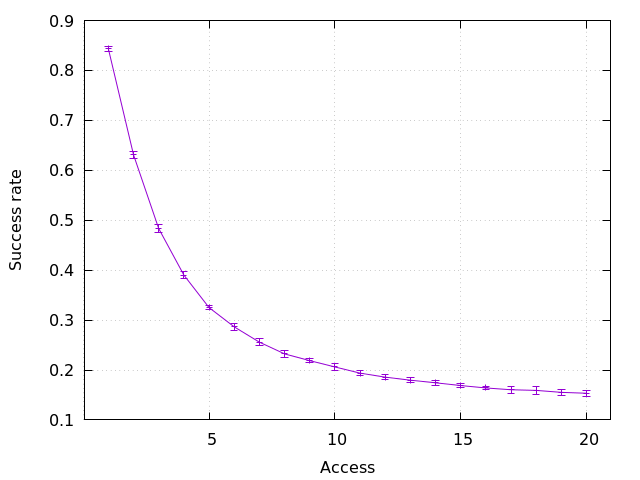
\includegraphics[width=.8\linewidth]{exp2/a/fig.png}
\end{figure}

\subsection{Experiment 3}

The next experiment modifies the server and client to allow a execution in 
separate machines. The experiments were carried out in the same physical 
machine, but in different erlang nodes.

The two nodes are named Alice and Bob, respectively assigned to run the Client 
and the Server. Two instances are required to run the experiment. The script 
\texttt{exp3/src/run.sh} launches first the node Alice. Then the module opty is 
started in Bob, which launches the Server locally, and starts the clients in the 
node Alice.

By removing the comments to print the node in each module, we can see the 
following trace:

\begin{verbatim}
$ echo '1, 10, 10, 10, 3' | ./run.sh | sort | uniq
Running configuration 1, 10, 10, 10, 3
1, 10, 10, 10, 3, 1, 0.9995698924731182
Client runs on node alice@127.0.0.1
Handler runs on node alice@127.0.0.1
Server runs on node bob@127.0.0.1
\end{verbatim}

Which shows that the server is running in one node, and the clients and handler 
in other node. We can observe the network communication by using 
\texttt{netstat}.

\begin{Verbatim}[fontsize=\scriptsize]
$ netstat -pn | grep erl
tcp        0      0 127.0.0.1:45067         127.0.0.1:4369          ESTABLISHED 26499/erl
tcp      107      0 127.0.0.1:49585         127.0.0.1:38775         ESTABLISHED 26500/erl
tcp        0    107 127.0.0.1:38775         127.0.0.1:49585         ESTABLISHED 26499/erl
tcp        0      0 127.0.0.1:46049         127.0.0.1:4369          ESTABLISHED 26500/erl
unix  3      [ ]         STREAM     CONNECTED     164666   26537/erl_child_set
unix  3      [ ]         STREAM     CONNECTED     164665   26499/erl
unix  3      [ ]         STREAM     CONNECTED     166328   26500/erl
unix  3      [ ]         STREAM     CONNECTED     166329   26538/erl_child_set
\end{Verbatim}

\subsection{Experiment 4}

In the last experiment we are going to compare the Opty implementation with the 
timestamp ordering technique, Timey. All the experiments in the experiment 1 are 
going to be executed using Timey.

\paragraph{\texttt{exp4a}: Clients vs Success rate.}

Timey seems to behave better as the number of clients grow. We can see how the 
success rate with 20 clients is about 0.2, while in Opty is less than 0.1.

\begin{figure}[H]
\centering
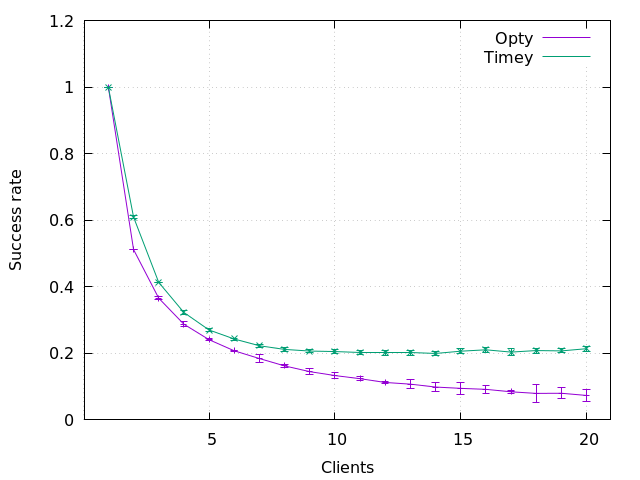
\includegraphics[width=.8\linewidth]{exp4/a/fig.png}
\end{figure}

\paragraph{\texttt{exp4b}: Entries vs Success rate}

As the number of entries grow, Timey seems to perform better up to 18, then Opty 
has a bigger success rate.
\nopagebreak
\begin{figure}[H]
\centering
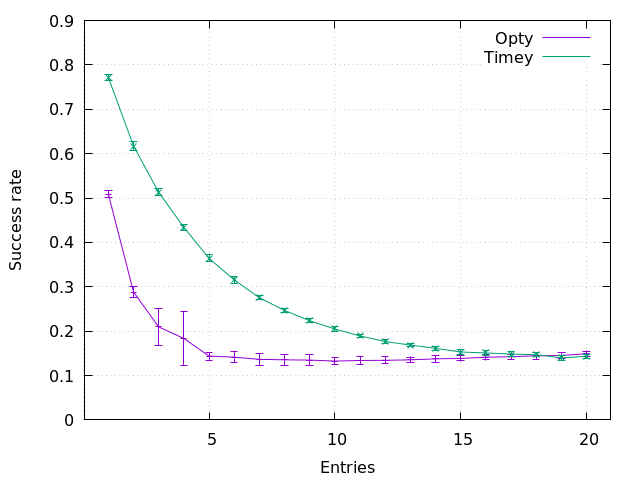
\includegraphics[width=.8\linewidth]{exp4/b/fig.png}
\end{figure}

\paragraph{\texttt{exp4c}: Reads vs Success rate}

Timey wins when the number of reads is greater than 5.

\nopagebreak
\begin{figure}[H]
\centering
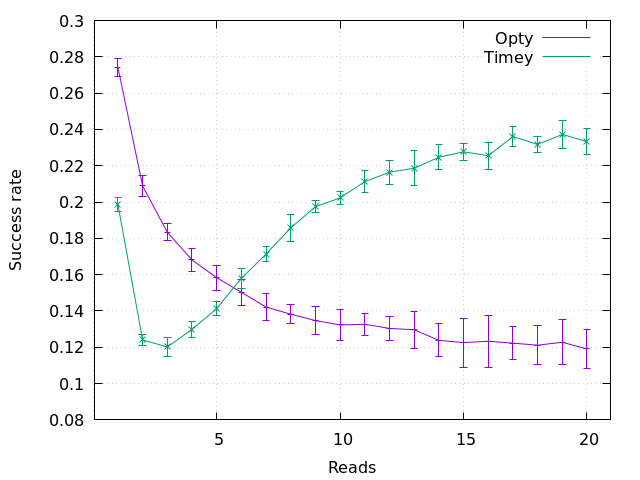
\includegraphics[width=.8\linewidth]{exp4/c/fig.png}
\end{figure}

\paragraph{\texttt{exp4d}: Writes vs Success rate}

For the writes, up to 20 Timey seems to perform better.

\nopagebreak
\begin{figure}[H]
\centering
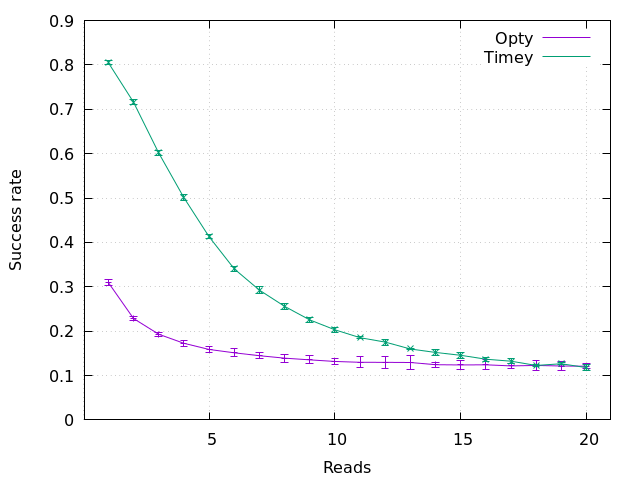
\includegraphics[width=.8\linewidth]{exp4/d/fig.png}
\end{figure}

\paragraph{\texttt{exp4e}: Time vs Success rate}

The deviation in the average success as the time grows seem to be small in both 
implementations.

\nopagebreak
\begin{figure}[H]
\centering
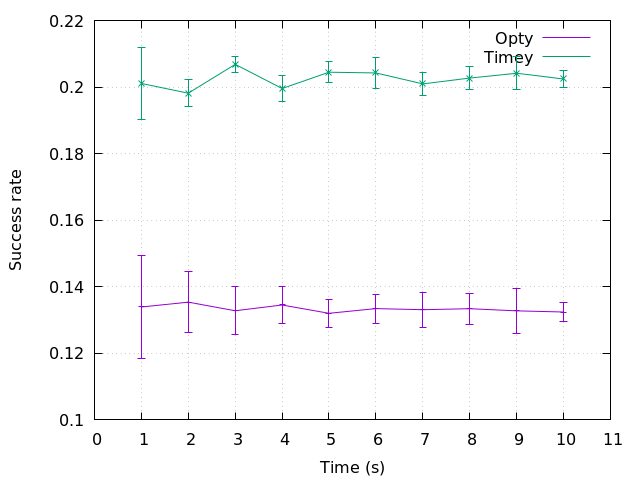
\includegraphics[width=.8\linewidth]{exp4/e/fig.png}
\end{figure}

\newpage
\paragraph{\texttt{exp4f}: Ratio R/W vs Success rate}

When the number of reads grows more than 7 reads (13 writes) then Timey starts 
to perform better than Opty.
\nopagebreak
\begin{figure}[H]
\centering
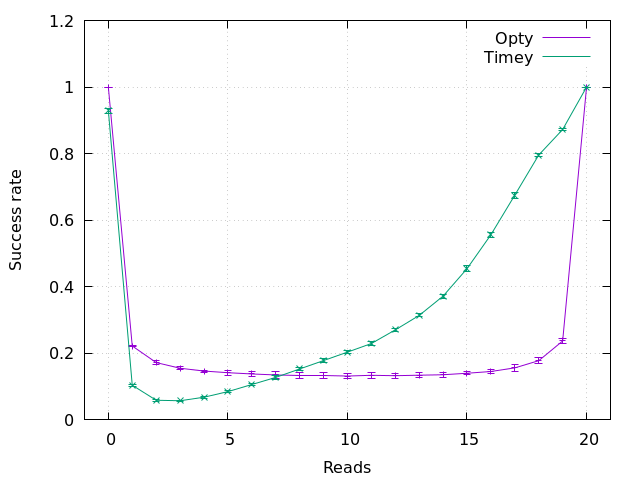
\includegraphics[width=.8\linewidth]{exp4/f/fig.png}
\end{figure}


\section{Remarks and conclusions}

First, the design of this experiment does not provide enough information to have 
a complete view of how both algorithm behave. As we are looking only at one 
variable at the time. A more careful experiment should take into account the 
effects in each parameter as a whole. A 2 factorial experiment could provide 
more useful information.

Also, the number of simulations is low, as the time taken by the algorithms is 
fixed to 3 seconds each datapoint. Lower times seem to increase the variance.

Finally, we can see that in some cases is better to choose the Timey algorithm 
over the Opty.

\section{Personal opinion}

Erlang is a bottleneck. I have spent about 90\% of the time figuring out how to 
instruct the language to do what I wanted. For example this kind of errors when 
something is wrong, are very hard to understand and to fix:

\begin{Verbatim}[fontsize=\scriptsize]
{"init terminating in do_boot",
{function_clause,[{lists,nth,[3,[]],[{file,"lists.erl"},{line,170}]},
{client,start,6,[{file,"client.erl"},{line,5}]},
{opty,startClients,7,[{file,"opty.erl"},{line,32}]},
{opty,start,5,[{file,"opty.erl"},{line,16}]},
{erl_eval,do_apply,6,[{file,"erl_eval.erl"},{line,670}]},
{init,start_it,1,[]},
{init,start_em,1,[]},
{init,do_boot,3,[]}]}}
\end{Verbatim}

Please look for a simpler alternative. Maybe Go is simple and stable enough. Or 
maybe you can provide a simple program with a graphical simulation to understand 
what happens.

\end{document}
